\documentclass[aspectratio=169]{beamer}

\usetheme{Madrid}
\usecolortheme{default}
\usepackage{graphicx}
\usepackage{booktabs}
\usepackage{array}

% Figures are stored in ./figures
\graphicspath{{figures/}}

\title{Device-Local Authorization for Secure Execution and Debug in Embedded Systems}
\subtitle{Master's Thesis Defense}
\author{[Your Name]}
\institute{[Department / University]}
\date{[Date]}

\begin{document}

\begin{frame}
  \titlepage
  \vspace{1ex}
  \centering
  \small Supervisor: [Supervisor Name]
\end{frame}

\begin{frame}{Outline}
  \begin{itemize}
    \item Motivation and problem
    \item Related work
    \item Methodology
    \item Implementation
    \item Experiments and results
    \item Conclusion and future work
  \end{itemize}
\end{frame}

\begin{frame}{Introduction}
  \begin{itemize}
    \item Embedded systems operate in critical and exposed environments.
    \item Physical access enables firmware replacement and invasive debug.
    \item Secure boot protects only the initial image.
    \item Post-boot authorization must be enforced on-device.
  \end{itemize}
\end{frame}

\begin{frame}{System Overview}
  \begin{columns}[T]
    \column{0.46\textwidth}
    \begin{itemize}
      \item Host toolchain and UART authorization sequence
      \item Protected NVM and comparator on-device
      \item FSM gates execution and debug enablement
    \end{itemize}
    \column{0.54\textwidth}
    \centering
    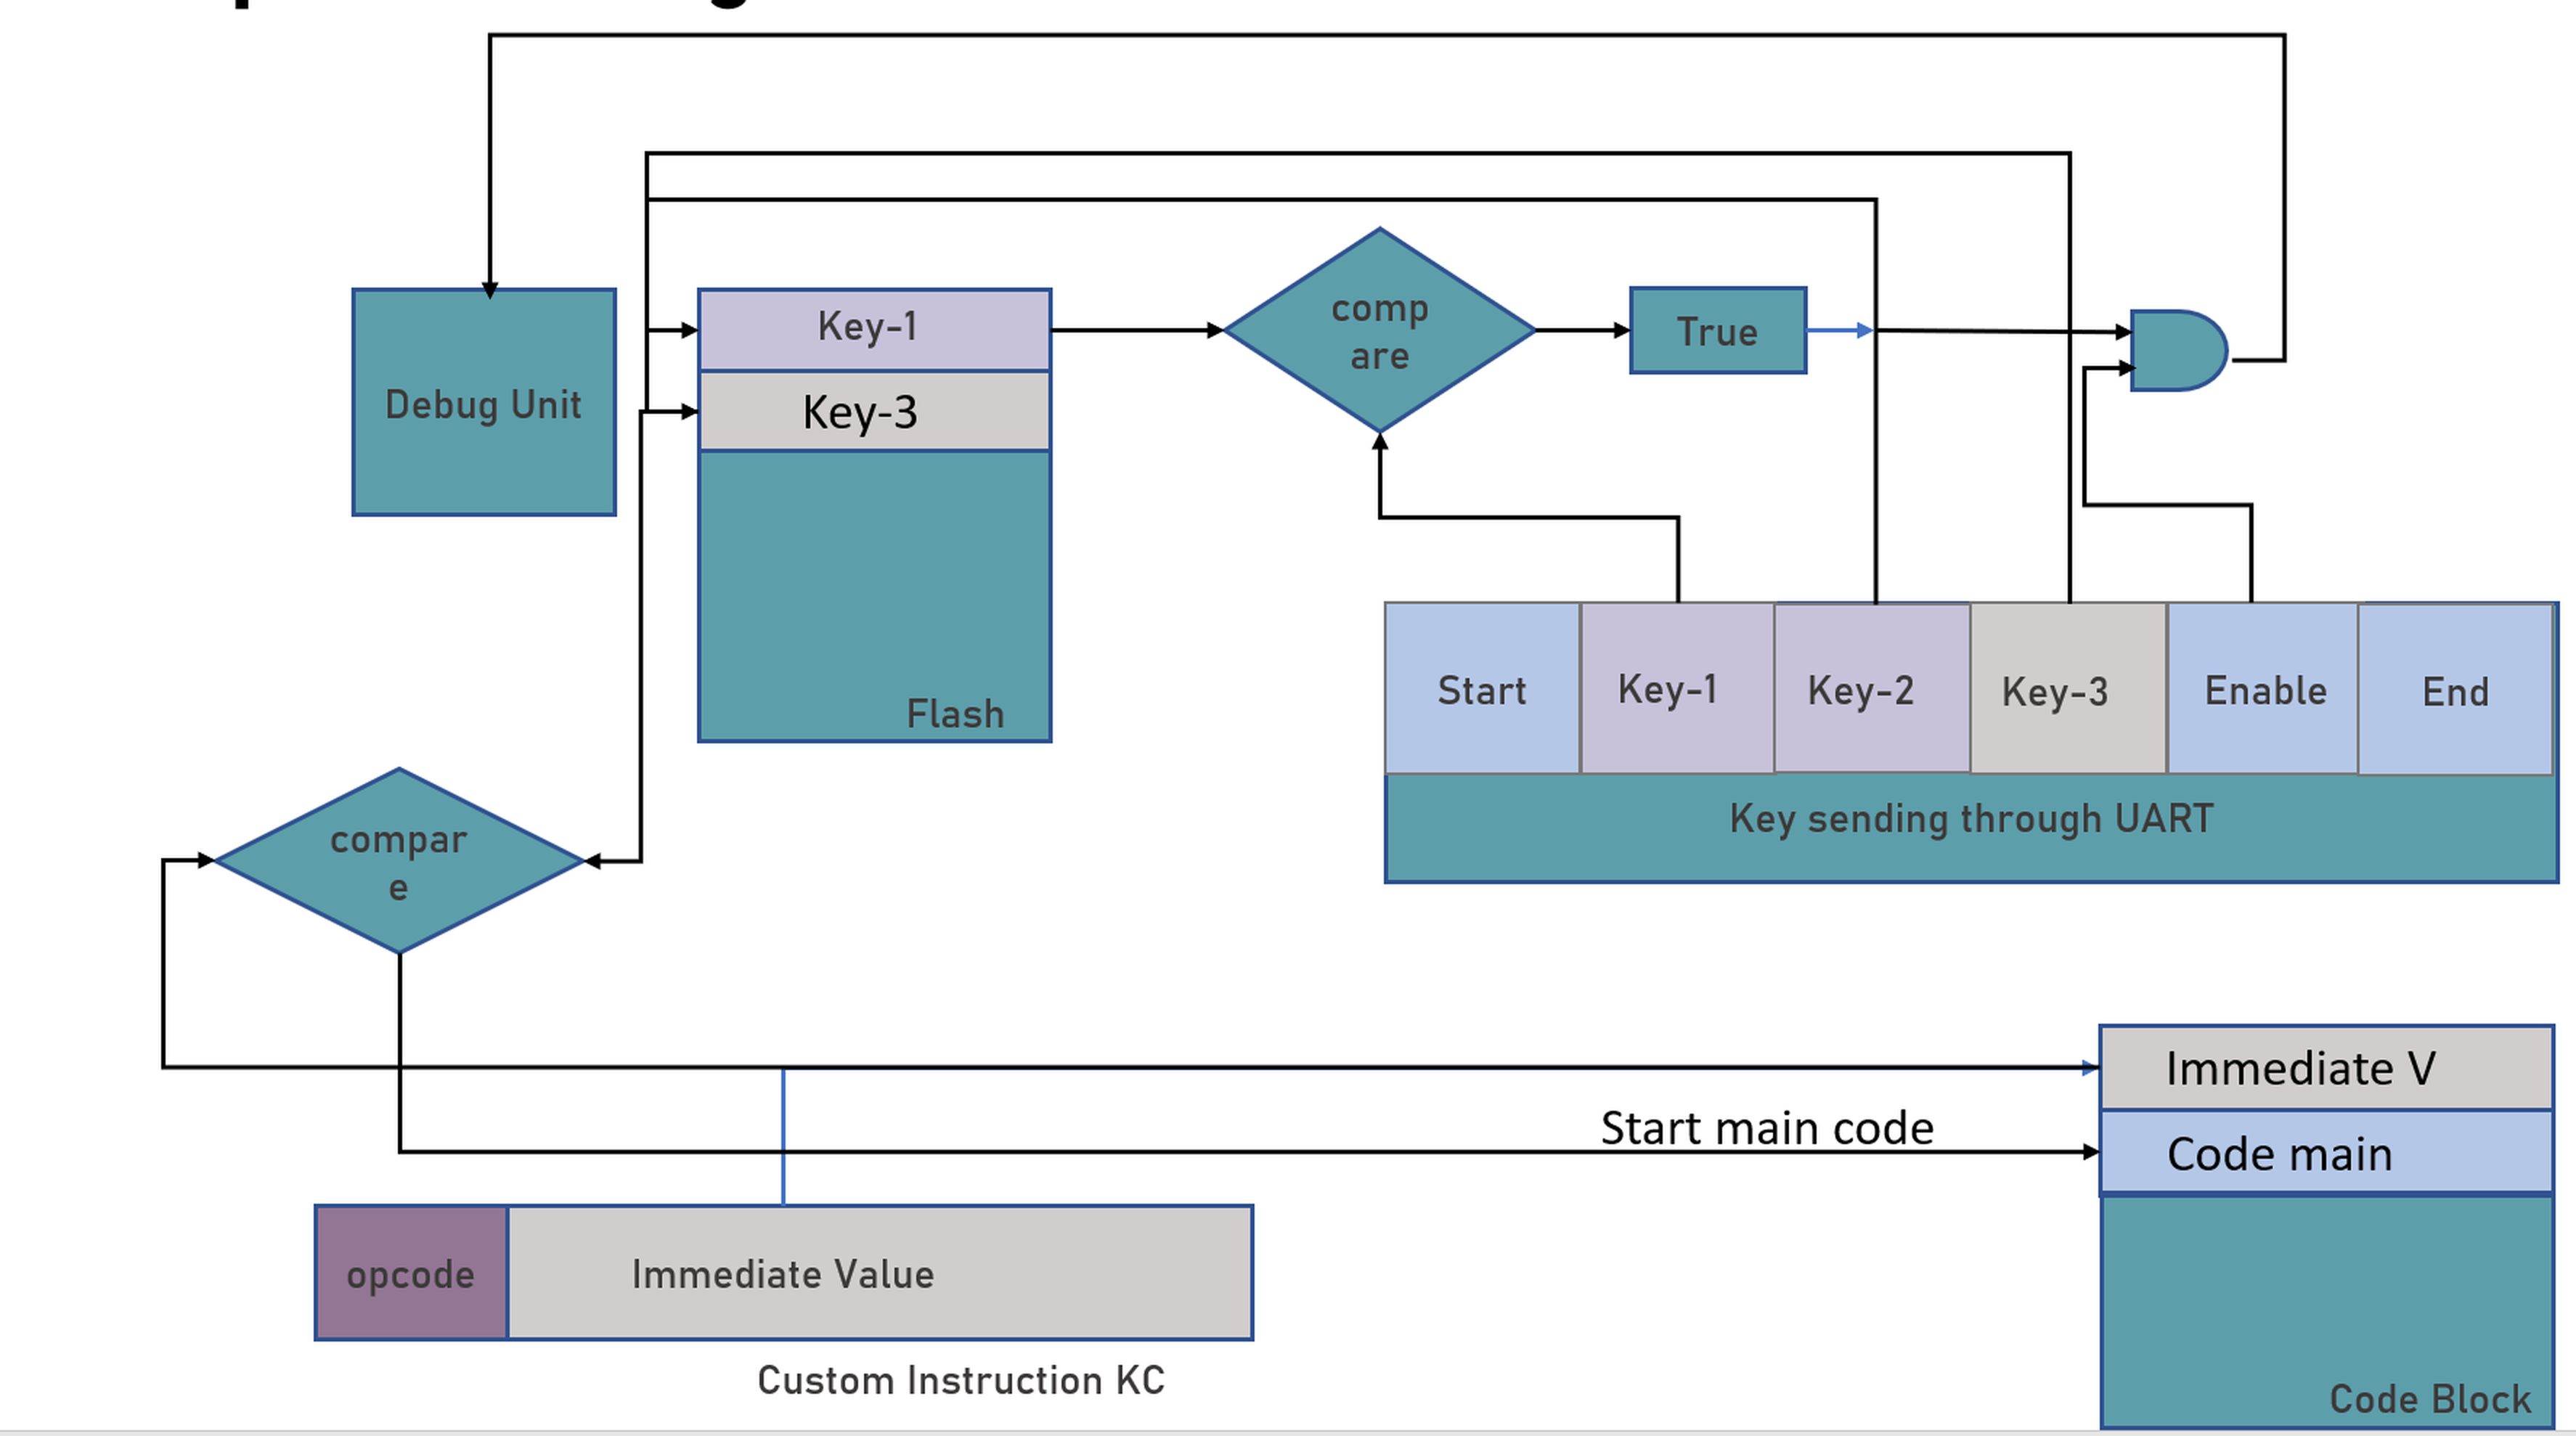
\includegraphics[width=\linewidth]{fig_arch_flow.png}
  \end{columns}
\end{frame}

\begin{frame}{Problem Statement}
  \begin{itemize}
    \item Post-boot debug/program access can bypass policy.
    \item Key material must not be exposed via normal memory.
    \item Host-side controls are insufficient after reflashing.
  \end{itemize}
\end{frame}

\begin{frame}{Key Contributions}
  \begin{itemize}
    \item ISA-level authorization trigger (\texttt{kc})
    \item Protected key storage with constant-time comparison
    \item FSM gating with fail-stop behavior
    \item Toolchain and host workflow integration
  \end{itemize}
\end{frame}

\begin{frame}{Related Work}
\end{frame}

\begin{frame}{Secure Boot and Boot-Chain Protection}
  \begin{itemize}
    \item BootROM validates initial firmware image.
    \item Boot-chain protection extends integrity across stages.
    \item Post-boot authorization still required.
  \end{itemize}
\end{frame}

\begin{frame}{Debug Interface Security}
  \begin{itemize}
    \item JTAG and test interfaces provide invasive access.
    \item Authenticated debug reduces exposure.
    \item Need execution-bound authorization on-device.
  \end{itemize}
\end{frame}

\begin{frame}{Trusted Execution and Minimal TCB}
  \begin{itemize}
    \item TEEs and minimal TCB reduce trusted code.
    \item Isolation does not automatically gate debug.
    \item Authorization complements trusted execution.
  \end{itemize}
\end{frame}

\begin{frame}{Runtime Attestation and CFI}
  \begin{itemize}
    \item Attestation provides evidence of runtime integrity.
    \item CFI/LO-FAT report control flow correctness.
    \item Evidence alone does not prevent debug misuse.
  \end{itemize}
\end{frame}

\begin{frame}{Software-Only Hardening}
  \begin{itemize}
    \item CFI, obfuscation, and ROP defenses add resistance.
    \item Software-only methods can be bypassed by reflashing.
    \item Hardware enforcement is required for strong control.
  \end{itemize}
\end{frame}

\begin{frame}{Toolchain and ISA Extensibility}
  \begin{itemize}
    \item LLVM enables analysis and instrumentation.
    \item RISC-V supports custom instruction extensions.
    \item Toolchain emission enables auditability.
  \end{itemize}
\end{frame}

\begin{frame}{Research Gap}
  \begin{itemize}
    \item Post-boot authorization not enforced on-device.
    \item Debug gating not tied to execution state.
    \item Need ISA-visible trigger with protected key storage.
  \end{itemize}
\end{frame}

\begin{frame}{Research Objectives}
  \begin{itemize}
    \item Define \texttt{kc} and the authorization protocol.
    \item Implement protected key storage and FSM gating.
    \item Integrate into toolchain and host workflow.
    \item Validate end-to-end enforceability.
  \end{itemize}
\end{frame}

\begin{frame}{Methodology}
\end{frame}

\begin{frame}{Overall Framework}
  \begin{itemize}
    \item Host derives key and sends UART sequence.
    \item Device verifies key with constant-time comparator.
    \item FSM releases execution and debug on match.
  \end{itemize}
\end{frame}

\begin{frame}{Key Derivation and Binding}
  \begin{itemize}
    \item Key derived from host and device identifiers.
    \item Nonce provides freshness.
    \item Reference stored in protected NVM.
  \end{itemize}
\end{frame}

\begin{frame}{Protected Key Storage}
  \begin{itemize}
    \item Not memory-mapped in normal address space.
    \item Accessible only via verification datapath.
    \item Comparator exposes only a match bit.
  \end{itemize}
\end{frame}

\begin{frame}{Authorization Sequence (UART)}
  \begin{itemize}
    \item Start, Key-1, Key-2, Key-3, Enable, End.
    \item Strict ordering and delimiter checks.
    \item Any mismatch triggers HALT.
  \end{itemize}
\end{frame}

\begin{frame}{Authenticator FSM and Gating}
  \begin{columns}[T]
    \column{0.5\textwidth}
    \begin{itemize}
      \item States: LOCKED, VERIFY, AUTHORIZED, HALT
      \item Reset begins in LOCKED
      \item VERIFY entered on \texttt{kc\_event}
    \end{itemize}
    \column{0.5\textwidth}
    \begin{itemize}
      \item match=1 $\rightarrow$ AUTHORIZED
      \item match=0 $\rightarrow$ HALT
      \item exec\_enable/debug\_enable only in AUTHORIZED
    \end{itemize}
  \end{columns}
\end{frame}

\begin{frame}{ISA Extension (\texttt{kc})}
  \begin{itemize}
    \item Custom I-type instruction
    \item Triggers verification datapath
    \item Binds authorization to execution point
  \end{itemize}
\end{frame}

\begin{frame}{Toolchain Integration}
  \begin{itemize}
    \item Compiler emits \texttt{kc} from C/assembly
    \item Linker preserves opcode placement
    \item ELF$\rightarrow$HEX keeps instruction
    \item Disassembly shows \texttt{kc} for audit
  \end{itemize}
\end{frame}

\begin{frame}{Authorization Dataflow}
  \begin{itemize}
    \item Provision key in protected NVM.
    \item Host sends UART sequence.
    \item Comparator validates fragments.
    \item FSM releases gates on match.
  \end{itemize}
\end{frame}

\begin{frame}{Experiments and Results}
\end{frame}

\begin{frame}{Evaluation Protocol}
  \begin{itemize}
    \item Functional validation over benchmarks.
    \item Verify \texttt{kc} preserved in build artifacts.
    \item Verify gating and fail-stop behavior.
  \end{itemize}
\end{frame}

\begin{frame}{Experimental Setup and Artifacts}
  \begin{itemize}
    \item Customized toolchain and host application.
    \item Device with protected NVM and FSM.
    \item Evidence from logs and screenshots.
  \end{itemize}
\end{frame}

\begin{frame}{Toolchain Validation}
  \centering
  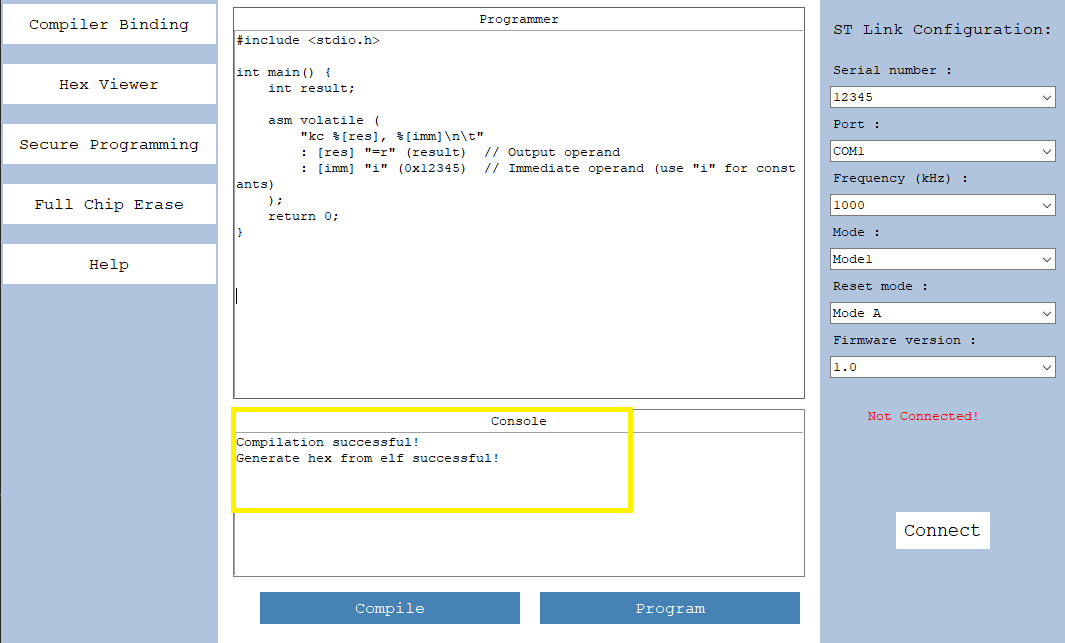
\includegraphics[width=0.92\linewidth]{fig_compile.png}
\end{frame}

\begin{frame}{Authorization Evidence}
  \begin{columns}
    \column{0.5\textwidth}
    \centering
    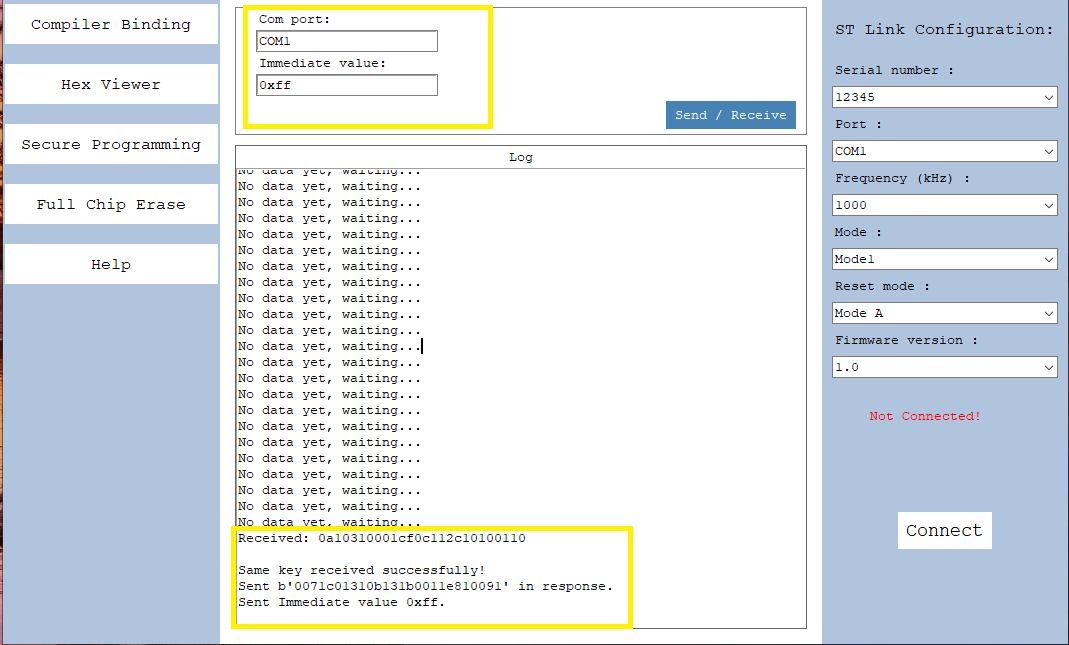
\includegraphics[width=\linewidth]{fig_keymatch.png}
    \column{0.5\textwidth}
    \centering
    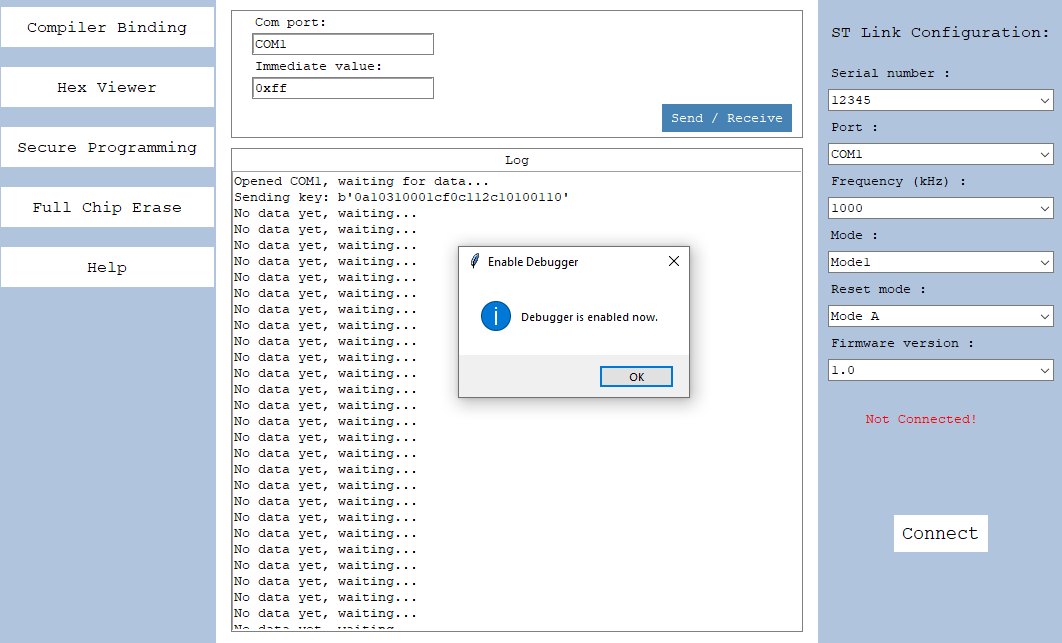
\includegraphics[width=\linewidth]{fig_debugenabled.png}
  \end{columns}
\end{frame}

\begin{frame}{Firmware Inspection and Fail-Stop}
  \begin{columns}
    \column{0.5\textwidth}
    \centering
    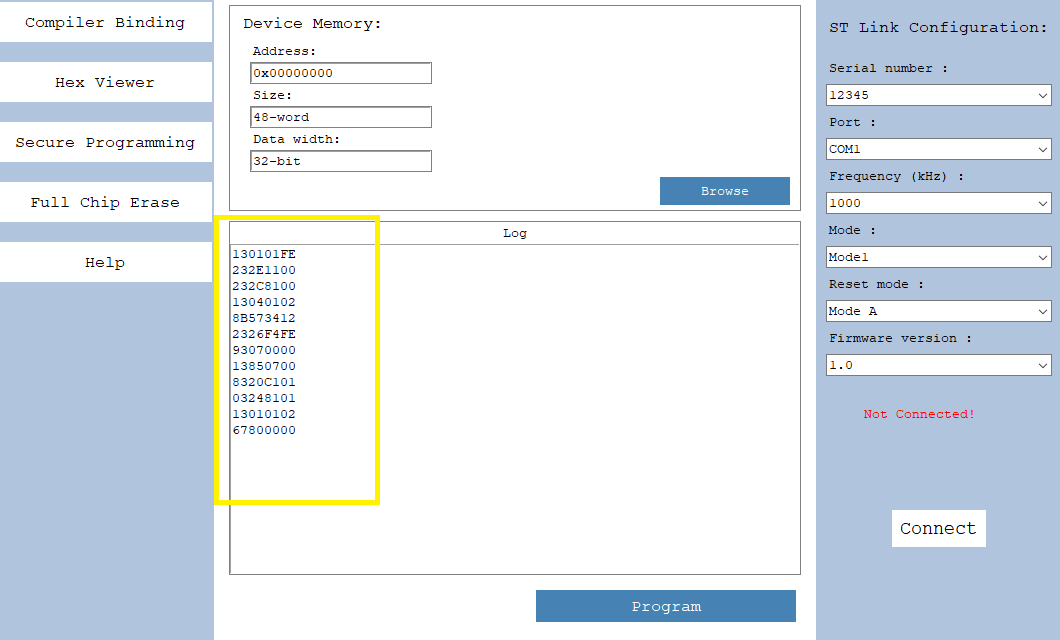
\includegraphics[width=\linewidth]{fig_hex.png}
    \column{0.5\textwidth}
    \centering
    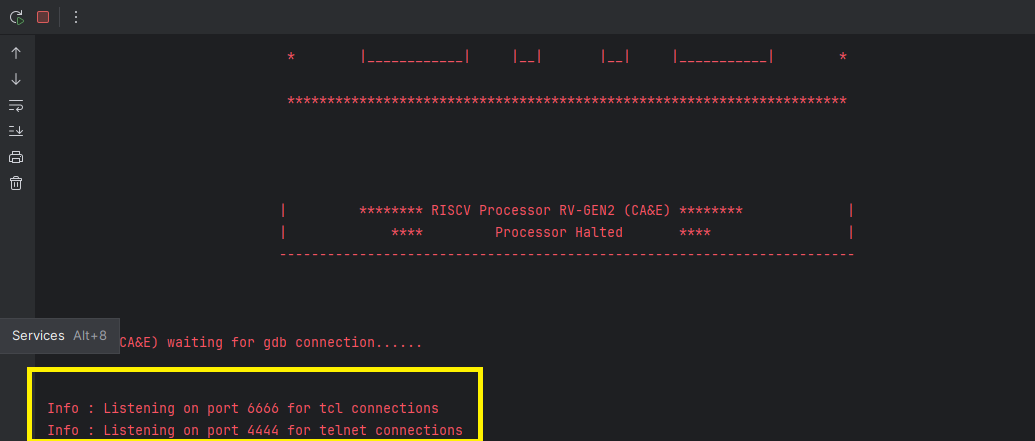
\includegraphics[width=\linewidth]{fig_halted.png}
  \end{columns}
\end{frame}

\begin{frame}{Programming Workflow Evidence}
  \begin{columns}
    \column{0.5\textwidth}
    \centering
    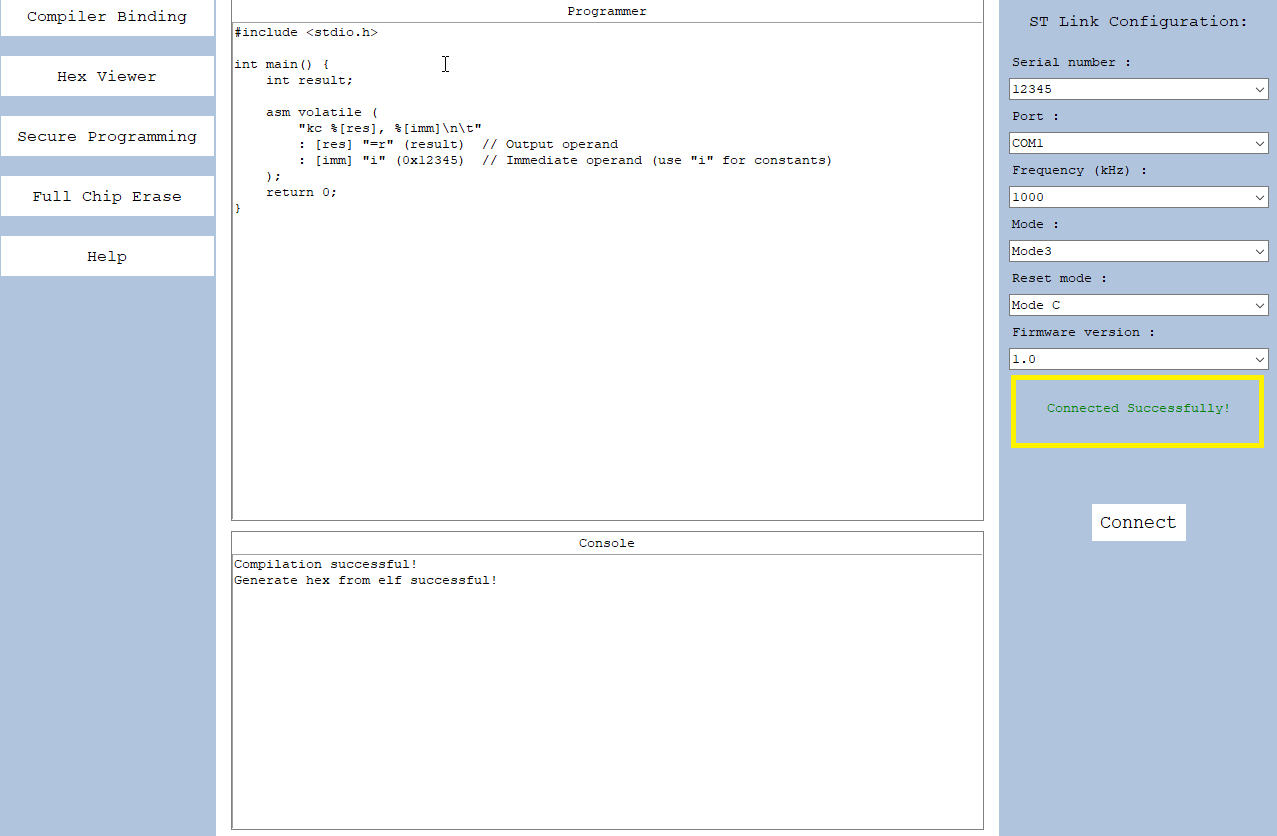
\includegraphics[width=\linewidth]{fig_connected.png}
    \column{0.5\textwidth}
    \centering
    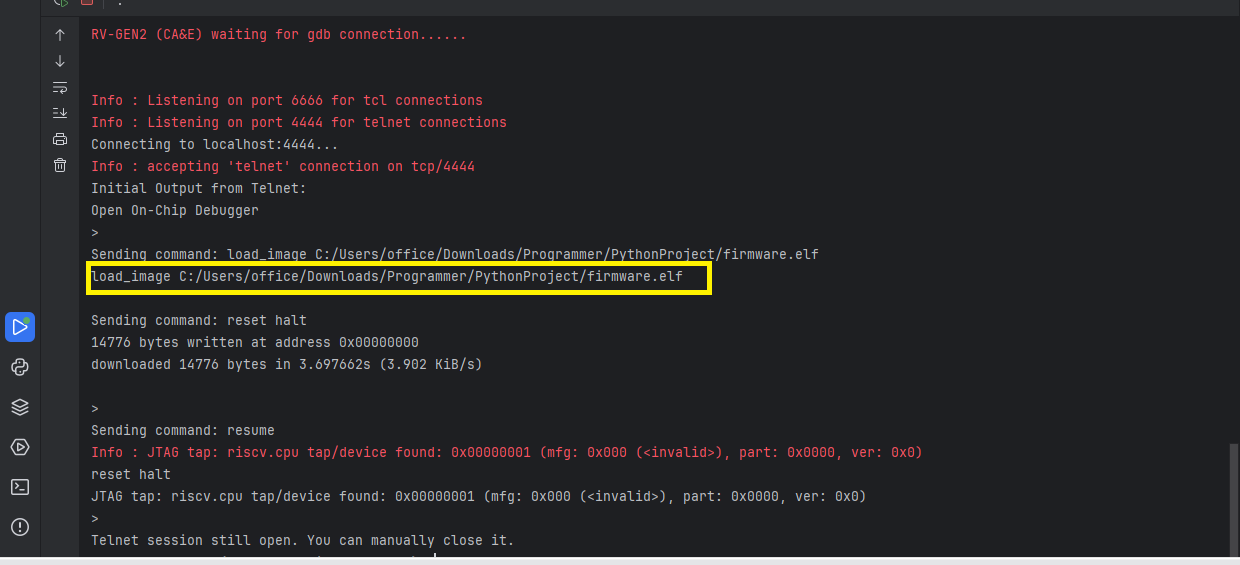
\includegraphics[width=\linewidth]{fig_loadimage.png}
  \end{columns}
\end{frame}

\begin{frame}{Conclusion}
\end{frame}

\begin{frame}{Conclusion}
  \begin{itemize}
    \item Device-local authorization closes the post-boot gap.
    \item Minimal ISA extension and protected storage are practical.
    \item Toolchain integration enables auditability.
  \end{itemize}
\end{frame}

\begin{frame}{Future Work}
  \begin{itemize}
    \item Measure area, power, and latency overheads.
    \item Key rotation and revocation policies.
    \item Fault and side-channel evaluation.
    \item Formal verification of FSM and toolchain tests.
  \end{itemize}
\end{frame}

\begin{frame}{References}
  \begin{itemize}
    \item IEEE Std 1149.1 (JTAG)
    \item BootROM secure boot design (Bin et al., 2020)
    \item JTAG authentication IP (Lapeyre et al., 2022)
    \item RISC-V ISA Manual (Waterman et al., 2014)
    \item C-FLAT control-flow attestation (Abera et al., 2016)
  \end{itemize}
\end{frame}

\begin{frame}{Questions}
  \centering
  {\Large Thank you}
\end{frame}

\end{document}
